
\section{Ladungen im Elektromagnetischen Feld
\label{relativ:section:em_feld}}
\rhead{Ladungen im Elektromagnetischen Feld}


\subsection{Elementarteilchen in der Relativitätstheorie
\label{relativ:section:elementarteilchen}}

Wie bereits in der Einleitung zu Abschnitt~\ref{relativ:section:relativistik} erwähnt,
kann es gemäss der Relativitätstheorie keine starren Körper geben.
Angemessener ist daher die Betrachtung \emph{punktförmiger Elementarteilchen}.
Der Zustand eines solchen Elementarteilchens ist dabei vollständig definiert durch
die drei Raumkoordinaten und die drei zugehörigen Geschwindigkeitskomponenten.


\subsection{Wirkungsintegral
\label{relativ:section:wirkungsintegral}}

Das Wirkungsintegral für ein Elementarteilchen im elektromagnetischen Feld ist
\begin{equation}
    S = \int_a^b \left(-mc\,ds + \frac{e}{c} \mathbf{A}\,d\mathbf{r} - e\varphi\,dt\right).
    \label{relativ:eqn:wirk-int-em-feld}
\end{equation}
Dabei ist \(\mathbf{A}\) das \emph{Vektorpotential des Feldes}\footnote{
    Auch bekannt als \emph{magnetisches Vektorpotential}.}
und \(\varphi\) das \emph{skalare potential des Feldes}\footnote{
    Auch bekannt als \emph{elektrisches Potential}.}.
In der relativistischen Raumzeit schreibt man diese zwei Grössen
auch als Vierervektor \(A^i = (\varphi, \mathbf{A})\),
wobei \(\varphi\) zur Zeitkoordinate \(t\) gehört und
\(\mathbf{A}\) zu den räumlichen Koordinaten \(x, y, z\).
Als Integral über die Zeit geschrieben ergibt sich das Wirkungsintegral als
\begin{equation}
    S = \int_{t_1}^{t_2} \biggl( -mc^2 \sqrt{1-\frac{v^2}{c^2}} + \frac{e}{c} \mathbf{A} \mathbf{v} - e \varphi \biggr) \, dt,
    \label{relativ:eqn:wirk-int-em-feld-zeit}
\end{equation}
wobei \(\displaystyle \mathbf{v} = \frac{d\mathbf{r}}{dt}\) der Geschwindigkeitsvektor der drei räumlichen Dimensionen ist.
Der Integrand in \eqref{relativ:eqn:wirk-int-em-feld-zeit} ist gerade die Lagrange-Funktion
\begin{equation}
    L = -mc^2 \sqrt{1-\frac{v^2}{c^2}} + \frac{e}{c} \mathbf{A} \mathbf{v} - e \varphi
    \label{relativ:eqn:lagrange-em-feld}
\end{equation}


\subsection{Bewegungsgleichung
\label{relativ:section:bewegungsgleichung}}

Bei der Berechnung der Bahn eines Elementarteilchens
in einem elektromagnetischen Feld geht man von
der vereinfachenden aber angemessenen Annahme aus,
dass die Rückwirkung des Teilchens auf das Feld vernachlässigt werden kann\footnote{
Konkret muss für diese Annahme beispielsweise
für die magnetische Feldstärke
\(H \ll \frac{m^2c^4}{e^3}\) erfüllt sein.
Die rechte Seite ergibt dabei für ein Elektron
eine magnetische Feldstärke von
\(\frac{m_e^2c^4}{e^3} \approx
\frac{(\qty{9e-31}{\kilogram})^2 (\qty{3e8}{\metre\per\second})^4}{(\qty{1.6e-19}{\ampere\second})^3}
\approx \qty[per-mode=fraction]{1.6e30}{\ampere\per\metre}\),
was im Vakuum einer magnetischen Flussdichte von
\(\mu_0 \cdot \qty[per-mode=fraction]{1.6e30}{\ampere\per\metre} \approx
\qty[per-mode=fraction]{1.25e-6}{\tesla\metre\per\ampere} \cdot
\qty[per-mode=fraction]{1.6e30}{\ampere\per\metre} =
\qty{2e24}{\tesla}\)
entspricht, einem Wert weitaus grösser als alle bekannten physikalischen Phänomene.}.

Die Bewegungsgleichung ergibt sich aus der Variation des Wirkungsintegrals
mit der Euler-Lagrange-Differentialgleichung
\begin{equation}
    \frac{d}{dt} \frac{\partial L}{\partial \mathbf{v}} - \frac{\partial L}{\partial \mathbf{r}} = 0,
    \label{realtiv:eqn:euler-lagrange-em-feld}
\end{equation}
wobei \(L\) in \eqref{relativ:eqn:lagrange-em-feld} gegeben ist.
Die Ableitung nach dem Geschwindigkeitsvektor \(\mathbf{v}\) ergibt
\begin{equation}
    \frac{\partial L}{\partial \mathbf{v}} =
    mc^2 \frac{-\frac{2}{c^2}\mathbf{v}}{-2\sqrt{1-\frac{v^2}{c^2}}}
    + \frac{e}{c} \mathbf{A} - 0
    = \frac{m \mathbf{v}}{\sqrt{1-\frac{v^2}{c^2}}} + \frac{e}{c} \mathbf{A}.
    \label{realtiv:eqn:part-diff-v}
\end{equation}
Dies wird auch als verallgemeinerter Teilchenimpuls \(\mathbf{P}\) bezeichnet,
wovon der linke Term der gewöhnliche (relativistische) Impuls \(\mathbf{p}\)
des Teilchens ist.

Die partielle Ableitung von \(L\) nach \(\mathbf{r}\) ergibt dann
\begin{equation}
    \frac{\partial L}{\partial \mathbf{r}} = \nabla L
    = 0 + \frac{e}{c} \operatorname{grad} \mathbf{Av} - e \operatorname{grad} \varphi.
    \label{realtiv:eqn:part-diff-r}
\end{equation}
Wir können nun \eqref{realtiv:eqn:part-diff-v} und \eqref{realtiv:eqn:part-diff-r}
in \eqref{realtiv:eqn:euler-lagrange-em-feld} einsetzen und erhalten
\begin{equation}
    \frac{d}{dt} \biggl(\mathbf{p} + \frac{e}{c} \mathbf{A}\biggr)
    - \frac{e}{c} \operatorname{grad} \mathbf{Av} + e \operatorname{grad} \varphi = 0.
    \label{realtiv:eqn:euler-lagrange-em-eingesetzt}
\end{equation}
Diese Differentialgleichung kann mittels Formeln der Vektoranalysis
umgeformt werden, um schliesslich
\begin{equation}
    \frac{d\mathbf{p}}{dt} = -\frac{e}{c} \frac{\partial\mathbf{A}}{\partial t}
    - e \operatorname{grad} \varphi +
    \frac{e}{c} \mathbf{v} \times \operatorname{rot} \mathbf{A}
    \label{realtiv:eqn:euler-lagrange-em-eingesetzt}
\end{equation}
zu erhalten.

\begin{beispiel}
\label{realtiv:bsp:teilchen-konst-e-feld}
Gehen wir von der einfachen Situation aus,
in der sich ein Elektron durch ein statisches
elektrisches Feld bewegt und \(\mathbf{A}\)
somit dem Nullvektor entspricht.
Der Geschwindigkeitsvektor des Elektrons sei
\(\mathbf{v}_0 = \mathbf{v}(t=0) =(\beta c, 0, 0)^T\), wobei
\(\beta \in (0, 1)\).
Die Differentialgleichung reduziert sich somit zu
\begin{equation}
    \frac{d\mathbf{p}}{dt} =
    - e \operatorname{grad} \varphi.
    \label{relativ:eqn:euler-lagrange-bsp-1}
\end{equation}
In einem nächsten Schritt wird für \(\mathbf{p}\)
wieder der Ausdruck in \eqref{realtiv:eqn:part-diff-v} eingesetzt,
womit
\begin{equation}
    \frac{d\mathbf{p}}{dt} =
    \frac{d}{dt} \Biggl(\frac{m_e}{\sqrt{1-\frac{v^2}{c^2}}} \mathbf{v}\Biggr) =
    - e \operatorname{grad} \varphi,
\end{equation}
mit der Elektronenmasse \(m_e\) und der Elementarladung \(e\).
Die Ableitung des Impulses entspricht somit lediglich
dem Gradienten des elektrischen Potentials, oder dem elektrischen Feld.
Der wesentliche Unterschied zur klassischen Mechanik ist hierbei
der bekannte relativistische Korrekturfaktor
\(\sqrt{1-\frac{v^2}{c^2}}\).

Die zeitliche Ableitung des Ausdrucks in der Klammer ist nicht ganz trivial,
da \(v^2=\sqrt{\mathbf{v}\cdot\mathbf{v}}\)
und somit natürlich auch von \(t\) abhängt.
Mittels Quotientenregel ergibt sich
\begin{multline*}
    \frac{d\mathbf{p}}{dt}
    = \frac{d}{dt} \Biggl(\frac{m_e \mathbf{v}}{\sqrt{1-\frac{v^2}{c^2}}}\Biggr)
    = \frac{m_e\frac{d\mathbf{v}}{dt}\sqrt{1-\frac{v^2}{c^2}}
    -m_e\mathbf{v}\cdot\frac{-\frac{\cancel{2}}{c^2}\mathbf{v}}{\cancel{2}\sqrt{1-\frac{v^2}{c^2}}}
    \frac{d\mathbf{v}}{dt}}{1-\frac{v^2}{c^2}}\\
    = m_e\frac{d\mathbf{v}}{dt}\frac{\biggl(1-\frac{v^2}{c^2}\biggr)^\frac{1}{2}
    +\frac{\mathbf{v}\cdot\mathbf{v}}{c^2} \biggl(1-\frac{v^2}{c^2}\biggr)^{-\frac{1}{2}}}
    {\biggl(1-\frac{v^2}{c^2}\biggr)^1}
    = m_e\frac{d\mathbf{v}}{dt}\frac{\biggl(1-\frac{v^2}{c^2}\biggr)^1
    +\frac{v^2}{c^2}}{\biggl(1-\frac{v^2}{c^2}\biggr)^\frac{3}{2}}
    = \frac{m_e}{\biggl(1-\frac{v^2}{c^2}\biggr)^\frac{3}{2}}\frac{d\mathbf{v}}{dt}.
\end{multline*}

Nehmen wir nun beispielsweise an,
dass das elektrische Feld lediglich eine \(x\)-Komponente hat,
sprich \( \operatorname{grad} \varphi = (E_x, 0, 0)^T \),
so ergibt sich für die Ableitung des Geschwindigkeitsvektors
\begin{equation}
    \frac{d}{dt}
        \begin{pmatrix}
            v_x \\
            v_y \\
            v_z
        \end{pmatrix} =
        - \frac{e \biggl(1-\frac{v^2}{c^2}\biggr)^\frac{3}{2}}{m_e}
        \begin{pmatrix}
            E_x \\
            0 \\
            0
        \end{pmatrix}.
    \label{relativ:eqn:bsp-abl-v-vec}
\end{equation}
Hierbei ist klar, dass sich die Geschwindigkeitskomponenten
in \(y\)- und \(z\)-Richtung nicht ändern können.
Zusammen mit der Anfangsgeschwindigkeit \(\mathbf{v}_0\)
ergibt sich somit die nichtlineare Differentialgleichung erster Ordnung
\begin{equation}
    \frac{dv_x}{dt} = - \frac{e E_x}{m_e} \biggl(1-\frac{v_x^2}{c^2}\biggr)^\frac{3}{2}
\end{equation}
für die Geschwindigkeit in \(x\)-Richtung \(v_x\).
Diese kann mittels Separierung gelöst werden.
Wir separieren nach den Variablen \(v_x\) und \(t\)
und integrieren auf beiden Seiten:
\begin{align*}
    \int\frac{dv_x}{\biggl(1-\frac{v_x^2}{c^2}\biggr)^\frac{3}{2}}
    &= \int-\frac{e E_x}{m_e}dt \\
    \Rightarrow\quad\frac{v_x}{\sqrt{1-\frac{v_x^2}{c^2}}}
    &= -\frac{e E_x}{m_e}t + K_1.
\end{align*}
Diese Gleichung kann nun (etwas mühsam) nach \(v_x\) aufgelöst werden:
\begin{align*}
    \frac{v_x^2}{1-\frac{v_x^2}{c^2}}
    &= \biggl(-\frac{e E_x}{m_e}t + K_1\biggr)^2\\
    \Leftrightarrow\quad v_x^2 &= \biggl(-\frac{e E_x}{m_e}t + K_1\biggr)^2
    \biggl(1-\frac{v_x^2}{c^2}\biggr)\\
    \Leftrightarrow\quad
    v_x^2 \biggl(1 + \frac{1}{c^2}\biggl(-\frac{e E_x}{m_e}t + K_1\biggr)^2\biggr)
    &= \biggl(-\frac{e E_x}{m_e}t + K_1\biggr)^2\\
    \Leftrightarrow\quad
    v_x^2 &= \frac{\biggl(-\frac{e E_x}{m_e}t + K_1\biggr)^2}
    {1 + \frac{1}{c^2}\biggl(-\frac{e E_x}{m_e}t + K_1\biggr)^2}\\
    \Leftrightarrow\quad
    v_x(t) &= \frac{-\frac{e E_x}{m_e}t + K_1}
    {\sqrt{1+\biggl(-\frac{eE_x}{m_e c}t+\frac{K_1}{c}\biggr)^2}}.
\end{align*}
Und mit der Anfangsbedingung \(v_x(t=0)=\beta c\) erhält man
\begin{multline*}
    v_x(0) = \beta c = \frac{K_1}{\sqrt{1+\biggl(\frac{K_1}{c}\biggr)^2}}\quad
    \Leftrightarrow\quad K_1^2 = \beta^2 c^2 \Biggl(1+\Biggl(\frac{K_1}{c}\Biggr)^2\Biggr)\\
    \Leftrightarrow\quad K_1^2 (1-\beta^2) = \beta^2 c^2\quad
    \Leftrightarrow\quad K_1 = \frac{\beta c}{\sqrt{1-\beta^2}}
\end{multline*}
und somit eine vollständige Gleichung für die Geschwindigkeit des Elektrons.
In Abbildung~\ref{relativ:fig:elektron-em-feld} ist die Gleichung für einige
Werte von \(\beta\) und \(E_x\) dargestellt.
\begin{figure}
    \centering
    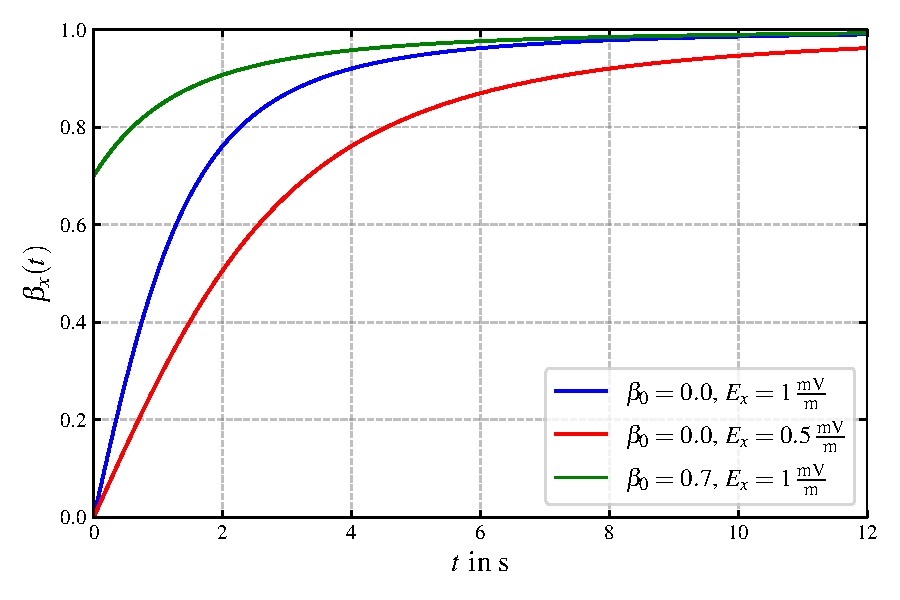
\includegraphics[width=0.8\linewidth]{papers/relativ/images/elektron_e-feld.pdf}
    \caption{Geschwindigkeit eines Elektrons in einem
    statischen elektrischen Feld in Abhängigkeit der Zeit \(t\),
    für verschiedene Feldstärken \(E_x\) und Startgeschwindigkeiten \(\beta c\).
    \label{relativ:fig:elektron-em-feld}}
\end{figure}

\todo{Erläuterungen}

\end{beispiel}
